\section{Sicherungsschicht}

\paragraph{Terminologie}
\begin{items}
  \item \textbf{Knoten}: Endsysteme + Router
  \item \textbf{Links}: Übertragungsabschnitt zwischen Knoten
  \item \textbf{Rahmen}: Pakete auf Schicht 2 (IP-Datagramme eingekapselt)
  \item \textbf{Aufgabe}: Übertraugng von Datagrammen zwischen benachbarten Knoten über Link
\end{items}

\paragraph{Aufgaben}
\begin{items}
  \item \textbf{Strukturierung} des Datenstroms (\emph{framing}) \\*
    \( \leadsto \) Datagramm in Rahmen einkapseln
  \item \textbf{Medienzugangskontrolle} bei geteilten Medien
  \item \textbf{Adressierung} mittels MAC-Adressen
  \item Je nach angebotenem Dienst \emph{Fehlererkennung/-behebung} bzw. \emph{Flusskontrolle}
  \item Übertragungsart: \\*
    - (Semi-) Broadbcast \\*
    - Punkt-zu Punkt (Halb-/Vollduplex)
\end{items}

\paragraph{Broadcast- vs. Punkt-zu-Punkt-Link}
\begin{items}
  \item \textbf{Broadcast-Link}: \\*
    alle Stationen können alle gesendeten Rahmen sehen (zB WLAN = semi-broadcast)
  \item \textbf{Punkt-zu-Punkt-Link}: \\*
    zwei Stationen sind über dedizierten Link verbunden (zB switch-basiertes Ethernet)
\end{items}

\paragraph{Punkt-zu-Punkt-Kommunikation}
\begin{items}
  \item \textbf{Simplex}: Übertragung in eine Richtung
  \item \textbf{Halbduplex}: Übertragung in beide Richtungen, nicht zeitgleich
  \item \textbf{(Voll-) Duplex}: Übertragung in beide Richtungen, zeitgleich
\end{items}

\paragraph{Sicherungsschicht --- Implementierung}
\begin{items}
  \item Sicherungsschicht ist in jedem Knoten (Endsystem, Router, Switch) implementiert (auf Netzadapter oder auf Chip), an Systembus angeschlossen (Kombination von Hardware, Software und Firmware)
\end{items}

\paragraph{Sicherungsschicht --- Kommunikation}
\begin{items}
  \item \textbf{Sender}: \\*
    - Datagramm einkapseln \\*
    - ggf Felder für Prüfsumme, Flusskontrolle etc hinzufügen
  \item \textbf{Empfänger}: \\*
    - Überprüfung hinsichtlich Fehler, Fluskontrolle usw \\*
    - Datagramm extrahieren und an Vermittlungsschicht weiterreichen
\end{items}

\paragraph{Sicherungsschicht --- Fehlererkennung}
\begin{items}
  \item \textbf{Wie Schicht 4}: Erkennung/Behebung von Bit- und Paketfehlern
  \item \textbf{Unterschied Schicht 4}: \\*
    - zu sendende/empfangende Bitfolge wird bitseriell betrachtet \\*
    - Internetprüfsumme basiert auf Wörtern, die bereits im Speicher stehen
  \item Rahmen erhält senderseitig Sicherungssequenz zur Überprüfung auf Empfangsseite \\*
    - \emph{frame check sequence} (FCS) \\*
    - steht üblicherweise an Rahmenende als Anhang
\end{items}

\paragraph{Fehlererkennung --- cyclic redundancy check (CRC)}
\begin{items}
  \item \textbf{Polynom}: \code{0101} \( \to 0x^3+1x^2+0x^1+1x^0 = x^2+1 \)
  \item \textbf{Generatorpolynom}: von \( g(x) \) generierte Code ist \\*
    \( C \coloneqq \{ v(x) \mid \text{deg}(v(x)) < n \wedge g(x) \text{ teilt } v(x) \} \)
  \item \textbf{Prinzip}: \\*
    - gleiches Polynom \( G(x) \) für Sender und Empfänger \\*
    - \emph{Sender}: \\*
    \phantom{-} \( \cdot \) hängt \( \text{deg}(G(x)) \) Nullen an Daten \\*
    \phantom{-} \( \cdot \) berechnet Rest von \( M(x)/G(x) \) (\( m \) Bit Rahmen \( \to M(x) \)) \\*
    \phantom{-} \( \cdot \) hängt Rest an mit Nullen erweiterte Daten an \\*
    - \emph{Empfänger}: Dividiert durch \( G(x) \) \\*
      \phantom{-} \( \cdot \) Ergebnis \( 0 \): keine Fehler erkannt \\*
      \phantom{-} \( \cdot \) Ergebnis \( \neq 0 \): Fehler!
\end{items}

\paragraph{CRC --- Wichtige Generatoren}
\begin{items}
  \item \textbf{CRC-12}: \( x^{12}+x^{11}+x^3+x^2+x+1 \)
  \item \textbf{CRC-16}: \( x^{16}+x^{15}+x^2+1 \)
  \item \textbf{CRC-CCITT}: \( x^{16}+x^{12}+x^5+1 \)
  \item \textbf{CRC-32}: \( x^{32}+x^{26}+x^{23}+x^{22}+x^{16}+x^{12}+x^{11}+x^{10}+x^8+x^7+x^5+x^4+x^2+x+1 \) 
\end{items}

\paragraph{CRC --- Hardwareimplementierung}
\begin{items}
  \item Rückgekoppelte Schieberegister \( \to \) CRC bei Durchschieben berechnet
  \item \textbf{Prinzip}: \\*
    - Bitweises Empfangen der Daten, durchlaufen Schieberegister \\*
    - Rückkopplung durch \code{XOR}-Gatter an 1-Stellen des Generators (ohne höchstes Bit)
\end{items}
\begin{figure}[H]\centering\label{Schieberegister}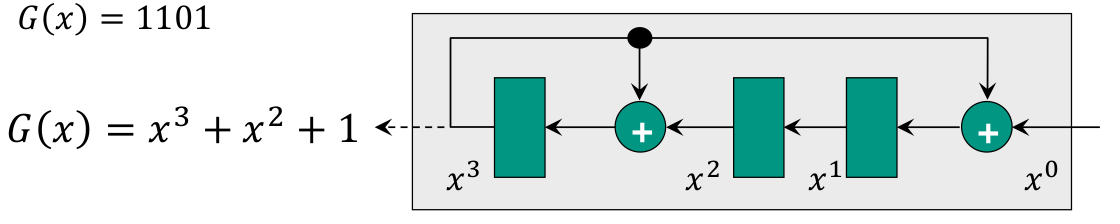
\includegraphics[width=0.33\textwidth]{Schieberegister}\end{figure}

\paragraph{Multiplexing}
\begin{items}
  \item \textbf{Problem}: Link von mehreren Knoten parallel benutzt
  \item \textbf{Dimensionen}: \\*
    - \emph{Raum} \( r \) \\*
    - \emph{Zeit} \( t \) \\*
    - \emph{Frequenz} \( f \) \\*
    - \emph{Code} \( c \)
  \item \textbf{Wichtig}: Schutzabstände erforderlich
\end{items}

\paragraph{Multiplexing --- Raum}
\begin{items}
  \item Raumeinteilung in Sektoren (zB gerichtete Antennen)
  \item \textbf{Kupfermultiplex}: Zuordnung dedizierter Leitungen
  \item \textbf{Einsatz}: Mobilfunkzellen
\end{items}

\paragraph{Multiplexing --- Frequenz}
\begin{items}
  \item \textbf{Prinzip}: verfügbare Bandbreite wird in Frequenzabschnitte unterteilt
  \item \textbf{Vorteile}: \\*
    - keine dynamische Koordination nötig \\*
    - auch für analoge Signale möglich
  \item \textbf{Nachteile}: \\*
    - Bandbreitenverschwendung bei ungleichmäßiger Auslastung \\*
    - unflexibel
  \item \textbf{Einsatz}: DSL
\end{items}

\paragraph{Multiplexing --- Zeit}
\begin{items}
  \item \textbf{Prinzip}: Kanal belegt ganzen Frequenzraum für festgelegte Zeit
  \item \textbf{Vorteile}: \\*
    - nur ein Träger gleichzeitig auf Medium \\*
    - auch bei großer Teilnehmerzahl hoher Durchsatz \\*
  \item \textbf{Nachteile}: \\*
    - genaue Synchronisation nötig
  \item \textbf{Einsatz}: Ethernet
  \item \textbf{Hinweis}: Standard-Multiplexverfahren im Folgenden
\end{items}

\paragraph{Multiplexing --- Code}
\begin{items}
  \item \textbf{Prinzip}: \\*
    - alle Stationen zur gleichen Zeit auf gleicher Frequenz \\*
    - \emph{Sender}: verknüpft Signal mit eindeutiger Pseudozufallszahl \\*
    - \emph{Empfänger}: kann mithilfe bekannter Pseudozufallszahlfolge + Korrelations- \\* \phantom{-} \phantom{\( \cdot \)} funktion Originalsignal wiederherstellen
  \item \textbf{Vorteile}: \\*
    - keine Frequenzplanung erforderlich \\*
    - großer Coderaum im Vergleich zu Frequenzraum \\*
    - Vorwärtskorrektur + Verschlüsselung leicht integrierbar
  \item \textbf{Nachteile}: \\*
    - höhere Komplexität wegen Signalregenerierung \\*
    - alle Signale müssen bei Empfänger gleich stark ankommen
  \item \textbf{Einsatz}: UMTS
\end{items}

\paragraph{Medienzugriff}
\begin{items}
  \item \textbf{Problem}: Unterschiedliche Medien (Kabel + Drahtlos)
  \item \textbf{Varianten}: \\*
    - feste Mediumszuteilung (feste Zeitschlitze, Punkt-zu-Punkt-Verbindungen) \\*
    - konkurrierende Nutzung \( \to \) Zugriffsorganisation notwendig
\end{items}

\paragraph{Zeitmultiplex --- Kategorien}
\begin{items}
  \item \textbf{fest}
  \item \textbf{variabel}: \\*
    - \emph{kontrollierter} Zugriff \\*
      \phantom{-} \( \cdot \) zentral \\*
      \phantom{-} \( \cdot \) dezentral \\*
    - \emph{zufälliger} Zugriff
\end{items}

\paragraph{Zeitmultiplex --- Zufallsstrategien}
\begin{items}
  \item \textbf{Aloha}: \\* 
    - verwendbar bei zufälligen, unabhängigen, seltenen Sendewünschen \\*
    - gleichzeitiges Senden \( \leadsto \) Kollision
  \begin{figure}[H]\centering\label{Aloha}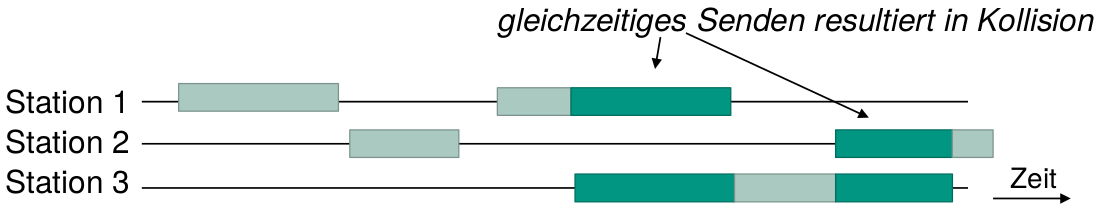
\includegraphics[width=0.33\textwidth]{Aloha}\end{figure}
  \item \textbf{Slotted Aloha}: \\*
    - Verbesserung von Aloha \\*
    - Erfordert Knotensynchronisation
    \begin{figure}[H]\centering\label{SlottedAloha}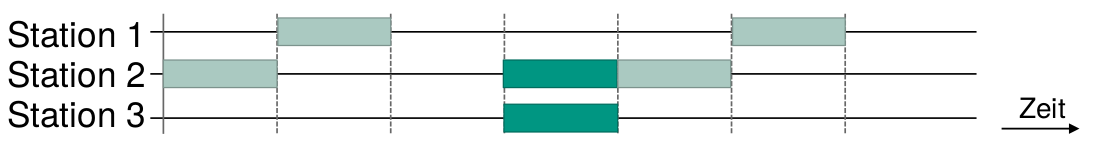
\includegraphics[width=0.33\textwidth]{SlottedAloha}\end{figure}
  \item \textbf{CSMA} (\emph{carrier sense multiple access}): \\*
    - \emph{Prinzip}: Andere nicht unterbrechen während sie reden \\*
    - \emph{listen before talk}: System prüft vor Senden, ob Medium frei ist \\*
    - \emph{Medium belegt}: später erneut versuchen \\*
    - \emph{Medium frei}: Senden \\*
    - \emph{Problem}: mehrere Systeme können quasi gleichzeitig Senden beginnen \\* \phantom{-} \phantom{\( \cdot \)} \( \leadsto \) Kollisionen
  \item \textbf{CSMA/CD} (\emph{CSMA with collision detection}) \\*
    - \emph{listen while talk}: Kollisionserkennung durch Abhören während des Sendens \\*
    - \emph{Kollision}: Sendungsabbruch, später neu versuchen
\end{items}

\paragraph{Zeitmultiplex --- Umsetzung Ethernet}
\begin{items}
  \item \textbf{Kollision}: \\*
    1. Sendungsabbruch \\*
    2. Sender sendet \emph{Jamming-Signal} \\*
    3. \emph{Backoff-Algorithmus} regelt Sendungswiederholung
  \item \textbf{Vorraussetzungen}: \\*
    - Senden der Rahmen darf nach Signallaufzeit durch Medium und zurück noch nicht \\* \phantom{-} \phantom{\( \cdot \)} fertig sein \\*
    - Mindestlänge für Rahmen (abhängig von Netzausdehnung + Ausbreitungsge- \\* \phantom{-} \phantom{\( \cdot \)} schwindigkeit) erforderlich \\*
    - zu kleiner Rahmen: Auffüllen auf Mindestlänge (\emph{padding})
\end{items}

\paragraph{Kollisionsfreier Zugriff --- Prinzip}
\begin{items}
  \item \textbf{Polling}: Kontrolle durch zentralen Knoten \\*
    - Senderecht sequentiell zugewiesen \\*
    - \emph{Nachteil}: koordinierender Knoten nötig, kann ausfallen \\*
    - \emph{Einsatz}: Bluetooth
  \item \textbf{Token Passing}: Senderechtsweitergabe von Knoten zu Knoten \\*
    - \emph{Nachteil}: Knoten können ausfallen \( \to \) Zugriff blockiert \\*
    - \emph{Einsatz}: Token Ring
\end{items}

\paragraph{Kollisionsfreier Zugriff --- Token Ring}
\begin{items}
  \item \textbf{Prinzip}: \\*
    - Systeme physikalisch Punkt-zu-Punkt-verbunden zu Ring \\*
    - Jedes System hat \emph{Vorgänger} und \emph{Nachfolger} \\*
    - Senderechtszuteilung durch zirkulierendes Token
\end{items}
\begin{figure}[H]\centering\label{TokenRing}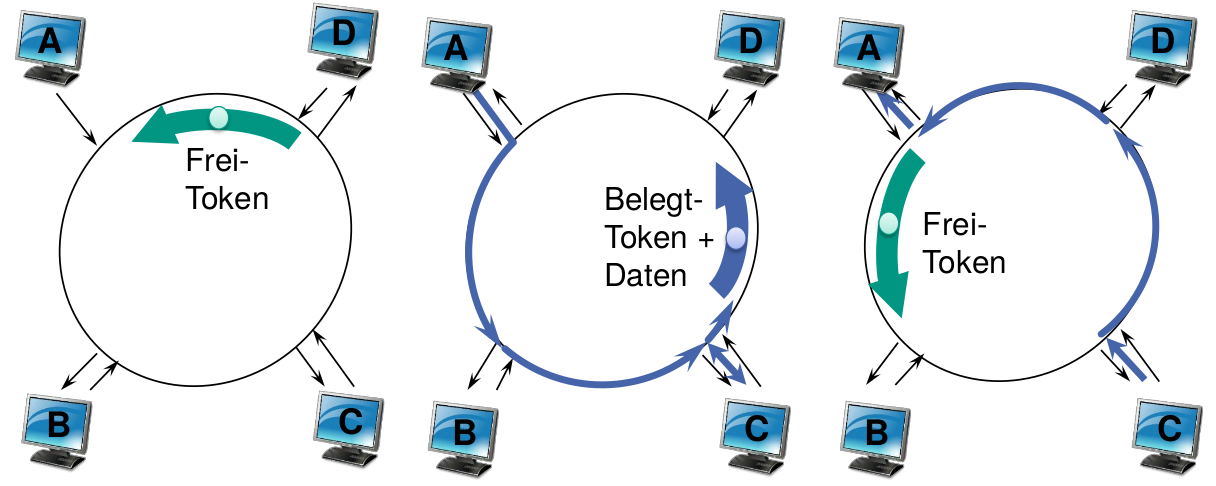
\includegraphics[width=0.33\textwidth]{TokenRing}\end{figure}

\paragraph{Kollisionsfreier Zugriff --- Token Bus}
\begin{items}
  \item \textbf{Prinzip}: \\*
    - Verbindet Vorteile von Ethernet und Token Ring \\*
    - Busverkabelung wie bei Ethernet \\*
    - \emph{Garantierte Antwortzeiten} durch zirkulierendes Token
  \item \textbf{Aufbau}: \\*
    - Alle Stationen physikalisch durch Bus verbunden \\*
    - Bildung eines \emph{logischen Rings}
\end{items}
\begin{figure}[H]\centering\label{TokenBus}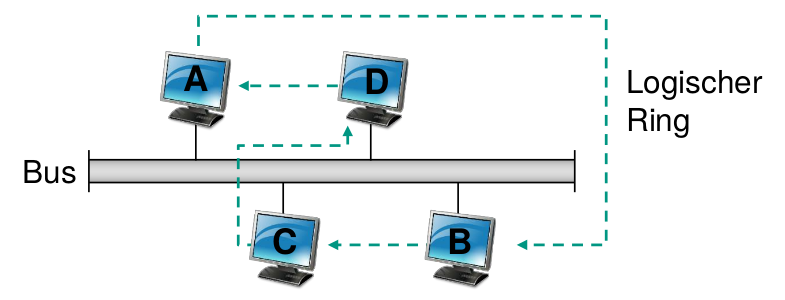
\includegraphics[width=0.33\textwidth]{TokenBus}\end{figure}

\paragraph{Lokale Netze --- MAC-Adressen}
\begin{items}
  \item Theoretisch weltweit eindeutig
  \item \textbf{Aufbau}: \\*
    - 24 Bit von IEEE an Hersteller zugewiesen \\*
    - 24 Bit von Hersteller durchnummeriert
  \item \textbf{Funktion}: lokal genutzt, um Rahmen von Interface zu benachbartem, physikalisch verbundenem Interface zu übertragen
  \item \textbf{Format}: \\*
    - 48 Bit \\*
    - stehen im NIC-ROM, können aber auch per Software gesetzt werden \\*
    - Darstellung meist hexadezimal (zB \code{24-2F-EA-76-CC-28}) \\*
    - Broadcast: \code{FF-FF-FF-FF-FF-FF}
\end{items}

\paragraph{Lokale Netze --- address resolution protocol (ARP)}
\begin{items}
  \item \textbf{Problem}: Welche MAC-Adresse hat nächstes System?
  \item \textbf{Aufgabe}: MAC-Adresse zu bekannter IP-Adresse ermitteln
  \item \textbf{Prinzip}: dynamisch Adresszuordnungen lernen
  \item \textbf{ARP-Cache}: kleine Tabelle auf jedem System \\*
    - Eintrag IP + MAC + maximale Lebenszeit \\*
    - Einträge bei Bedarf gelernt
\end{items}

\paragraph{ARP --- Adressauflösung}
\begin{items}
  \item \textbf{Szenario 1}: \( A \) sendet Datagramm an \( B \) in selbem Subnetz \\*
    - \emph{Fall 1}: ARP-Cache von \( A \) hat Eintrag für \( B \) \\*
      \phantom{-} \( \cdot \) Paket verschicken \\*
      \phantom{-} \( \cdot \) Timeout neu setzen \\*
    - \emph{Fall 2}: ARP-Cache von \( A \) hat Eintrag für \( B \) \emph{nicht}: \\*
      \phantom{-} \( \cdot \) Broadcast \emph{ARP-Request} mit IP von \( B \) \\*
      \phantom{-} \( \cdot \) Jeder Knoten liest ARP-Request --- falls eigene IP ARP-Reply \\*
      \phantom{-} \( \cdot \) \( A \) trägt Infos in ARP-Cache ein
  \item \textbf{Szenario 2}: \( A \) sendet Datagramm an \( B \) in anderem Subnetz \\*
    1. \( A \) sendet ARP-Request für Router \( R \) \\*
    2. \( A \) sendet Datagramm an IP von \( B \) und MAC von \( R \) \\*
    3. Router empfängt Datagramm, setzt Ziel-MAC auf \( B \) und Sender-MAC auf \( R \) \\*
    4. Router leitet Datagramm weiter
\end{items}

\paragraph{Lokale Netze --- Ethernet}
\begin{items}
  \item \textbf{Standard}: IEEE 802.3
  \item \textbf{Medienzuteilung}: \\*
    - zeitmultiplex, variabel, zufälliger Zugriff \\*
    - Verwendung von CSMA/CD (exponentieller Backoff) \\*
  \item \textbf{Netztopologie}: Ursprünglich Bus-, heute Sterntopologie
  \item \textbf{Varianten}: \\*
    - \emph{Bezeichnung}: [Datenrate][Baseband/Broadband][Medium] \\*
    - \emph{Invadiante}: Format Ethernet-Rahmen \\*
    - \emph{10Base5}: 10Mbit/s, Baseband, Bustopologie, 10mm Koax \\*
    - \emph{10Base2}: 10Mbit/s, Baseband, Bustopologie, 5mm Koax
\end{items}
\begin{figure}[H]\centering\label{EthernetVarianten}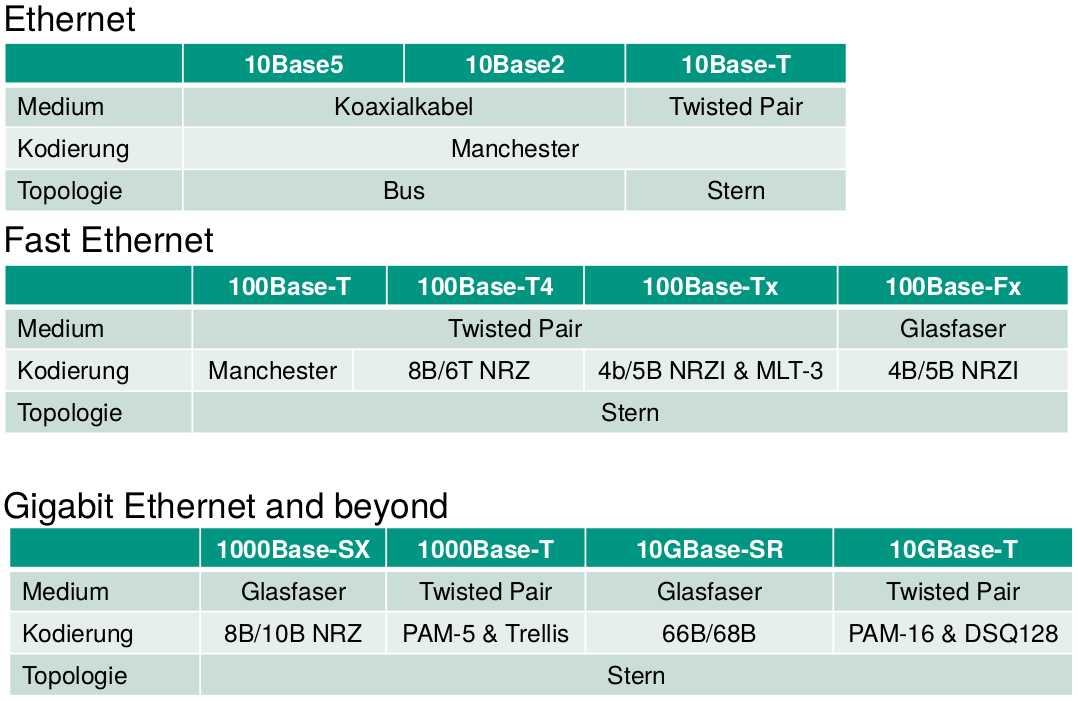
\includegraphics[width=0.33\textwidth]{EthernetVarianten}\end{figure}

\paragraph{Ethernet --- exponentieller Backoff}
\begin{items}
  \item \textbf{Schema}: Station wählt \emph{randomisiert} Anzahl zu wartender Zeitschlitze nach Schema: \\*
    - \emph{1. Kollision}: Wartezeit 0/1 Zeitschlitze \\*
    - \emph{2. Kollision}: Wartezeit 0/1/2/3 Zeitschlitze \\*
    - \emph{\( i \). Kollision}: Wartezeit 0/\dots/\( 2^i-1 \) Zeitschlitze \\*
    - \( i = 16 \) \( \leadsto \) Systemfehler
\end{items}

\paragraph{Ethernet --- Zeitschlitze}
\begin{items}
  \item \textbf{Prinzip}: \\*
    - Kanal wird logisch in Zeitschlitze fester Länge aufgeteilt \\*
    - Dauer = minimale Rahmenlänge \( \to \) Kollisionserkennung vor Zeitschlitz-Ende
\end{items}

\paragraph{Ethernet --- Switches}
\begin{items}
  \item \textbf{Prinzip}: \\*
    - Schicht-2-Netzkopplung \\*
    - Trennung von Inter- und Intranetz-Verkeht \( \to \) Erhöhung Netzkapazität \\*
    - Switches nicht sichtbar für Endsysteme
  \item \textbf{Ziel}: Selbstorganisierte Netzkonfiguration mit Switches
  \item \textbf{Aufgaben}: \\*
    - Etablierung schleifenfreie Netztopologie (\emph{spanning tree}) \\*
    - Etablierung von Wegen zwischen Endsystemen (selbstlernend)
\end{items}

\paragraph{Ethernet --- Kollisionsdomänen}
\begin{items}
  \item = Netzbereich, auf dem Kollision möglich ist
\end{items}
\begin{figure}[H]\centering\label{Kollisionsdomaenen}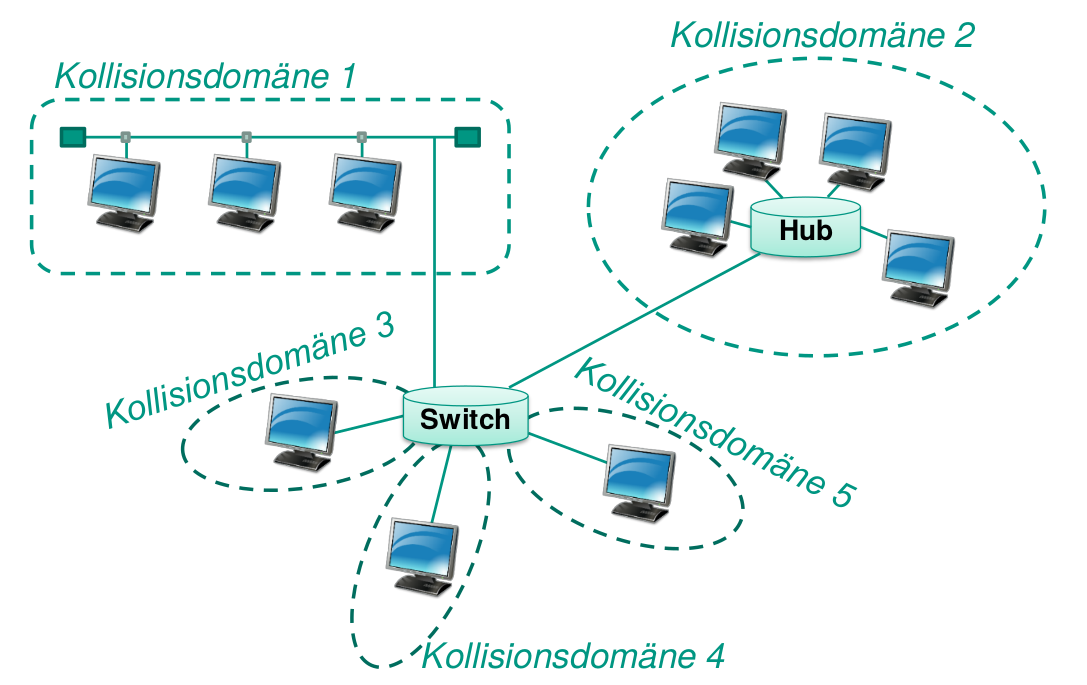
\includegraphics[width=0.33\textwidth]{Kollisionsdomaenen}\end{figure}

\paragraph{virtual local area network (VLAN)}
\begin{items}
  \item \textbf{Idee}: Logische Trennung von Datenverkehr auf Ethernet-Ebene \\* \( \leadsto \) virtuelle Leitung
  \item \textbf{Sicherheit}: \\*
    - Trennung in logische Medien ermöglicht gezielte Systemgruppierung \\*
    - Bessere Kontrolle über Netzstruktur
  \item \textbf{Flexibilität}: \\*
    - Einfache Reorganisation der logischen Medien möglich \\*
    - keine Änderungen an physikalischem Medium (Neuverkabelung) nötig
  \item \textbf{Performance}: Broadcast-Last eines Netzes sinkt, wenn physikalisches Medium in mehrere logische aufgeteilt wird
\end{items}

\paragraph{VLAN --- Interface-basiert}
\begin{items}
  \item \textbf{Verkehrsisolation}: Rahmen von Interfaces 1-8 können nur Interfaces 1-8 erreichen \\* \( \leadsto \) Sicherheit, Performance
  \item \textbf{Dynamische Zuweisung}: Interfaces dynamisch anderen VLANs zuordnern \\*
    \( \leadsto \) Flexibilität
  \item \textbf{Weiterleitung} zwischen VLANs über Routing (oft über in Switch integrierten Router)
  \item \textbf{Trunks}: Transport von Rahmen zwischen multi-switch-VLANs \\*
    - \emph{VLAN-ID}: Jedes VLAN erhält Kennzeichner \\*
    - Ethernet-Frames werden mit VLAN-ID getaggt \\*
    - Switches entfernen Tagging vor Auslieferung an Endsystem
\end{items}
\begin{figure}[H]\centering\label{VLAN}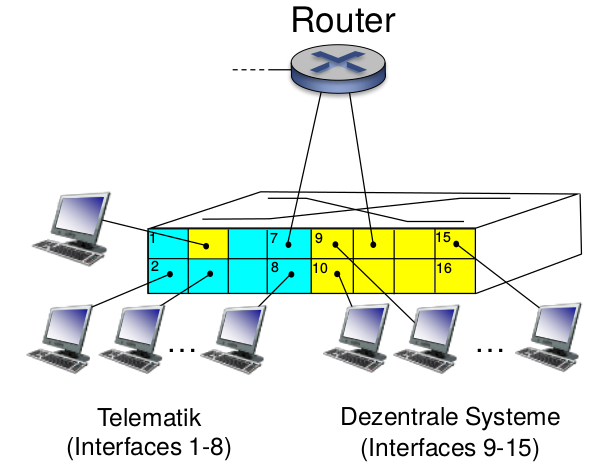
\includegraphics[width=0.33\textwidth]{VLAN}\end{figure}